\section{Gesamtkonzept}

\subsection{Visualisierung}

TODO SKIZZE


\subsection{Komponenten}

Folgendes Kompontenten fuer das Konzept wurden mithilfe der Technologierecherche (siehe Anhang \ref{techrecherche}) und anschliessenden morphologische Kästen (siehe Anhang \ref{mk}) und Nutzwertanalysen (siehe Anhang \ref{nutzwertanalyse}) ermittelt. 

\begin{table}[H]
\centering
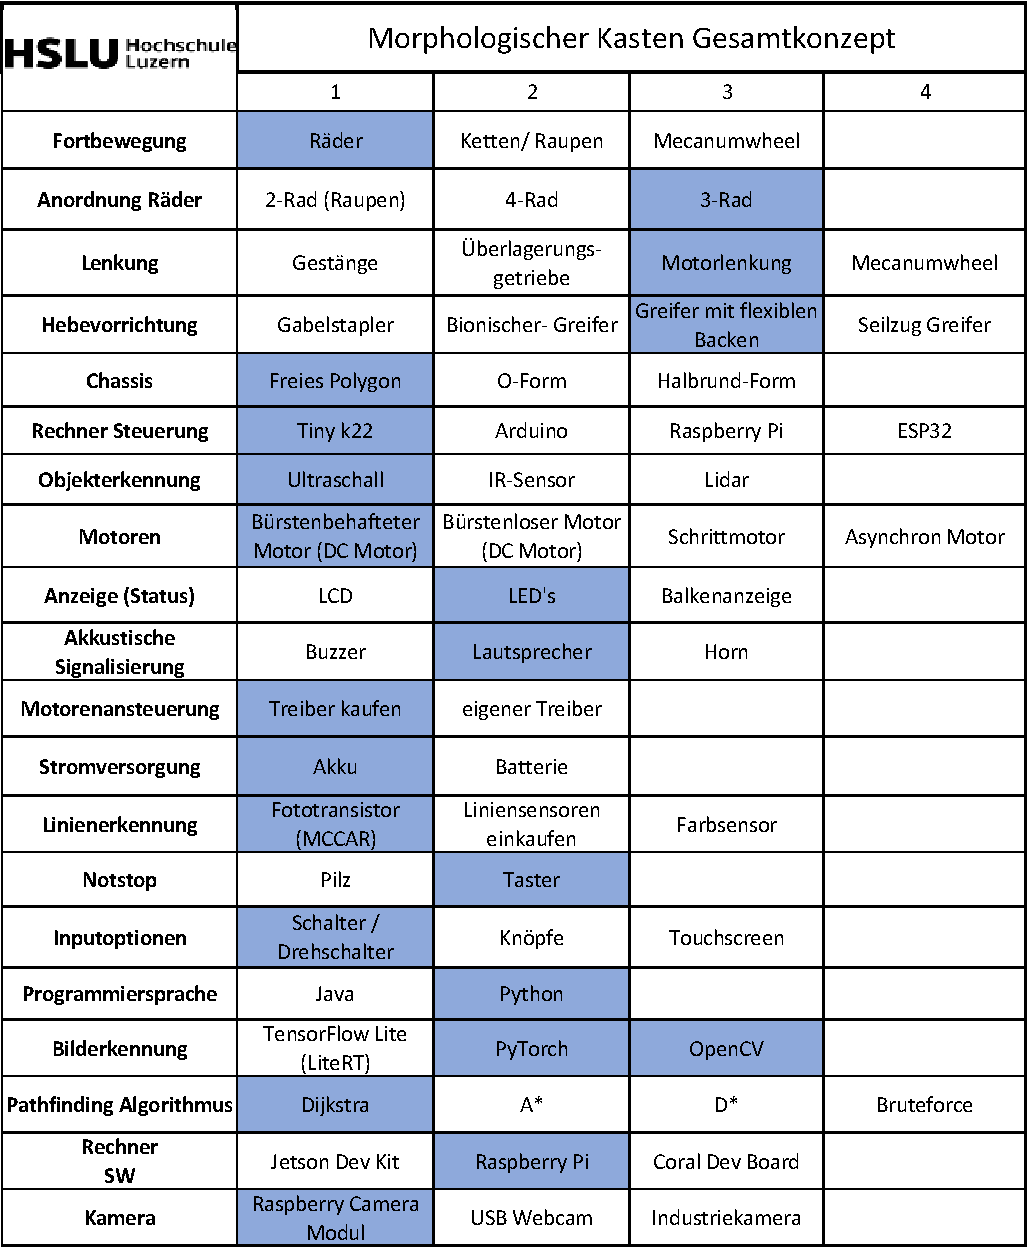
\includegraphics[width=\textwidth -20mm]{assets/MK-all.pdf}
\caption{Morphologischer Kasten: Gesamtkonzept}
\label{table:mk-all}
\end{table}

Es ist geplant einen Roboter in U-Form zu bauen, der sich mit drei Rädern fortbewegt und eine Motorlenkung besetzt. Hindernisse kann der Roboter mit einem Parallelgreifer anheben.

Die Steuerung wird auf einem Tiny k22 laufen. Die Distanz zu den Objekten wird mit Ultraschall erkannt. Die bürstenbehafteten Motoren werden mit einem gekauften Treiber angesteuert. Die Stromversorgung läuft über einen Akku. Der Akkustand und der Status des Roboters werden mit LED's angezeigt. Damit der Roboter die Linien erkennt, wird ein Liniensensor mit Fototransistoren verwendet. Das Ziel wird über einen Schalter vom Benutzer ausgewählt.
Wenn der Roboter das Ziel erreicht, verkündet er dies über einen Lautsprecher. Im Notfall wird der Roboter über einen Taster ausgeschaltet.

Die Software wird in Python geschrieben und läuft auf einem Raspberry Pi. Zur Bilderkennung wird eine Kombination von PyTorch und OpenCV verwendet. Die Bilder werden mit einer Raspberry Camera aufgenommen. Der kürzeste Weg wird mit einem Dijkstra Algorithmus berechnet.


\subsection{Ablauf}

Die Schritte, die mit einem Plus markiert sind, sind in den folgenden Kapiteln als Subprozesse detailliert definiert.

\begin{figure}[H]
\centering
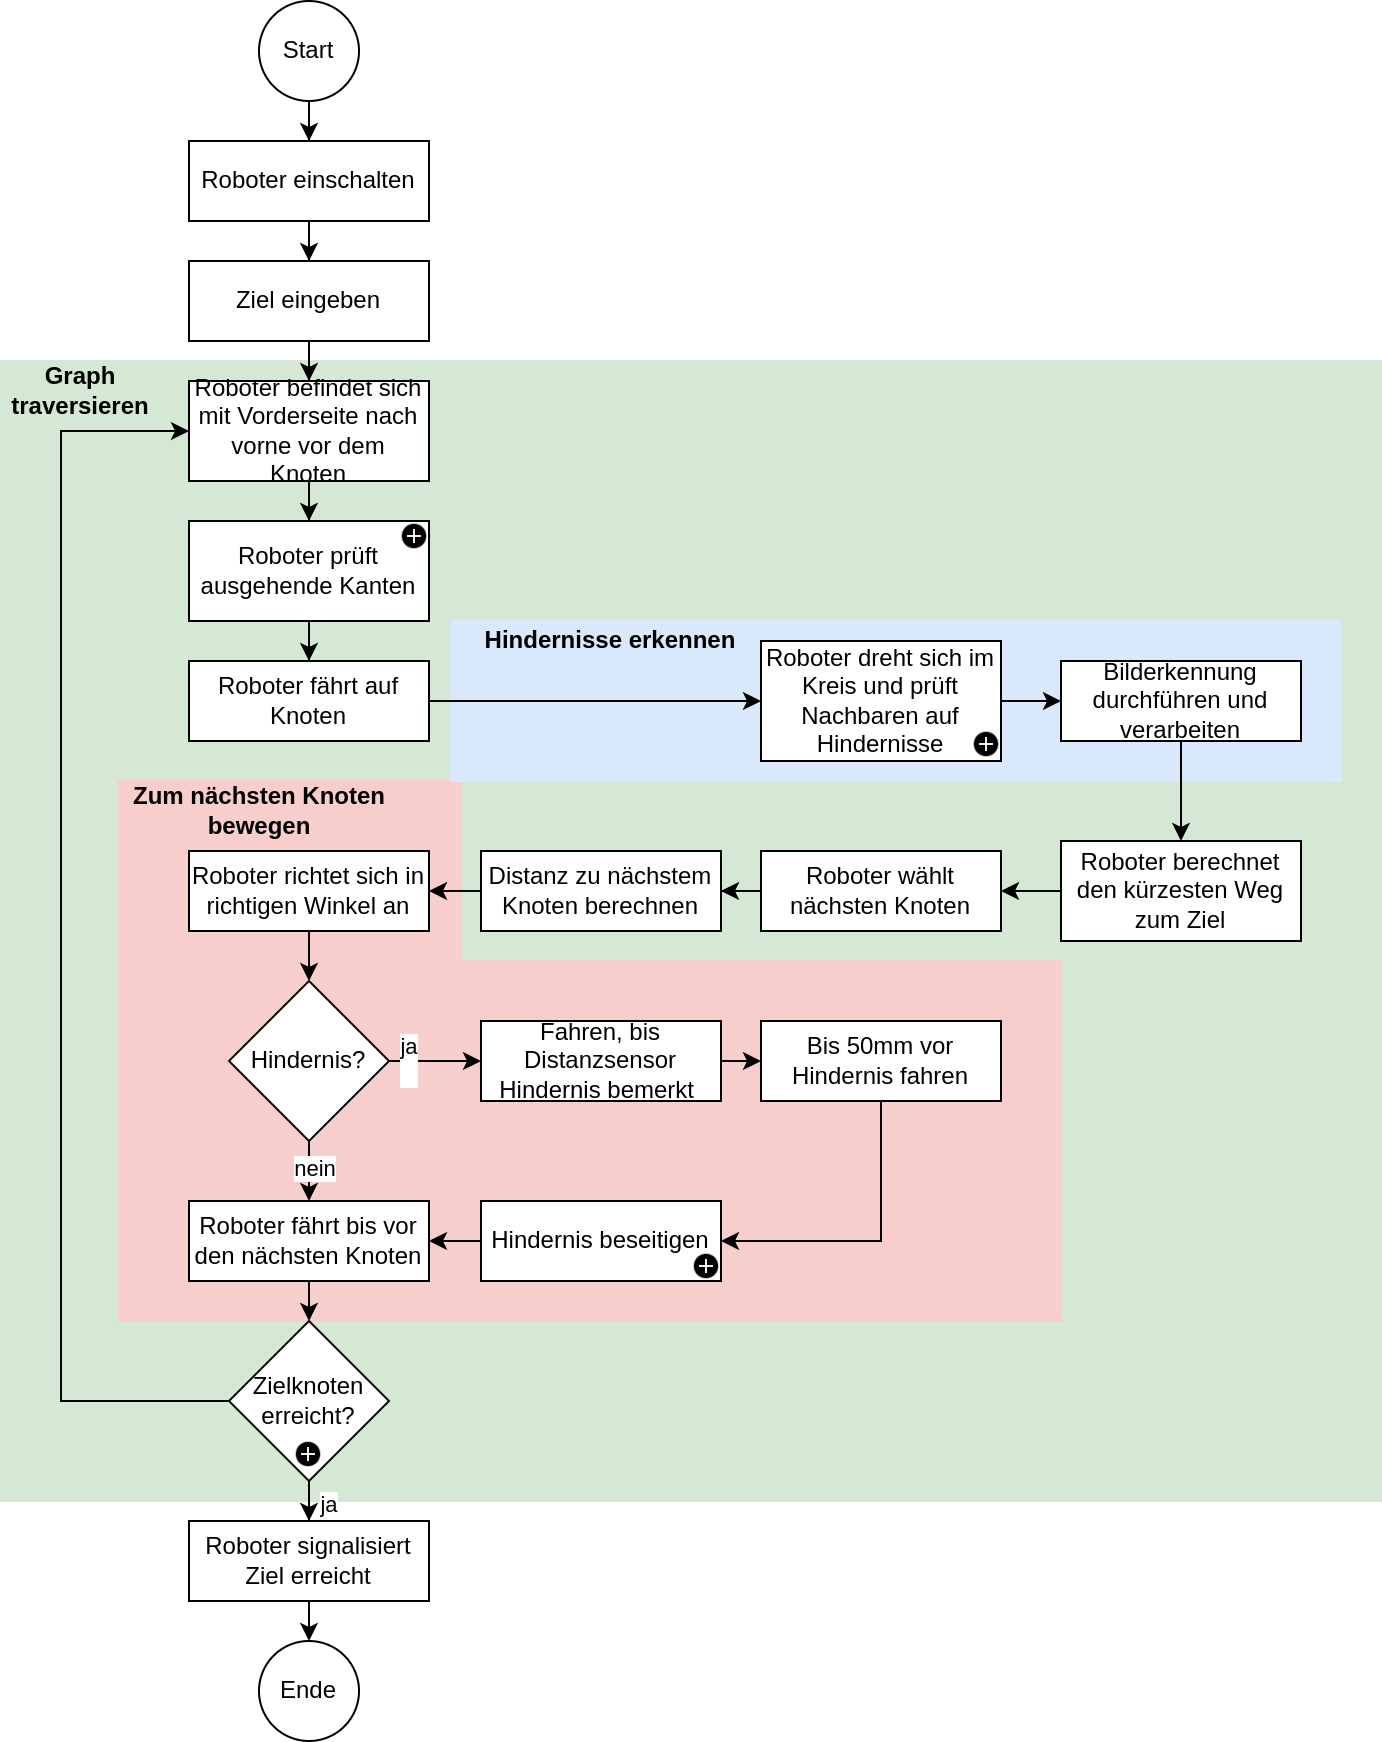
\includegraphics[width=\textwidth]{assets/gesamtkonzept/ablaufdiagramm.png}
\caption{Ablaufdiagramm}
\label{fig:ablaufdiagramm}
\end{figure}

\subsubsection{Fortbewegung}

PLACEHOLDER

\subsubsection{Linienerkennung}

PLACEHOLDER

\subsubsection{Kameraposition}

Hoehe \& Winkel, Hochformat

\subsubsection{Ausgehende Kanten erkennen}

\begin{figure}[H]
\centering
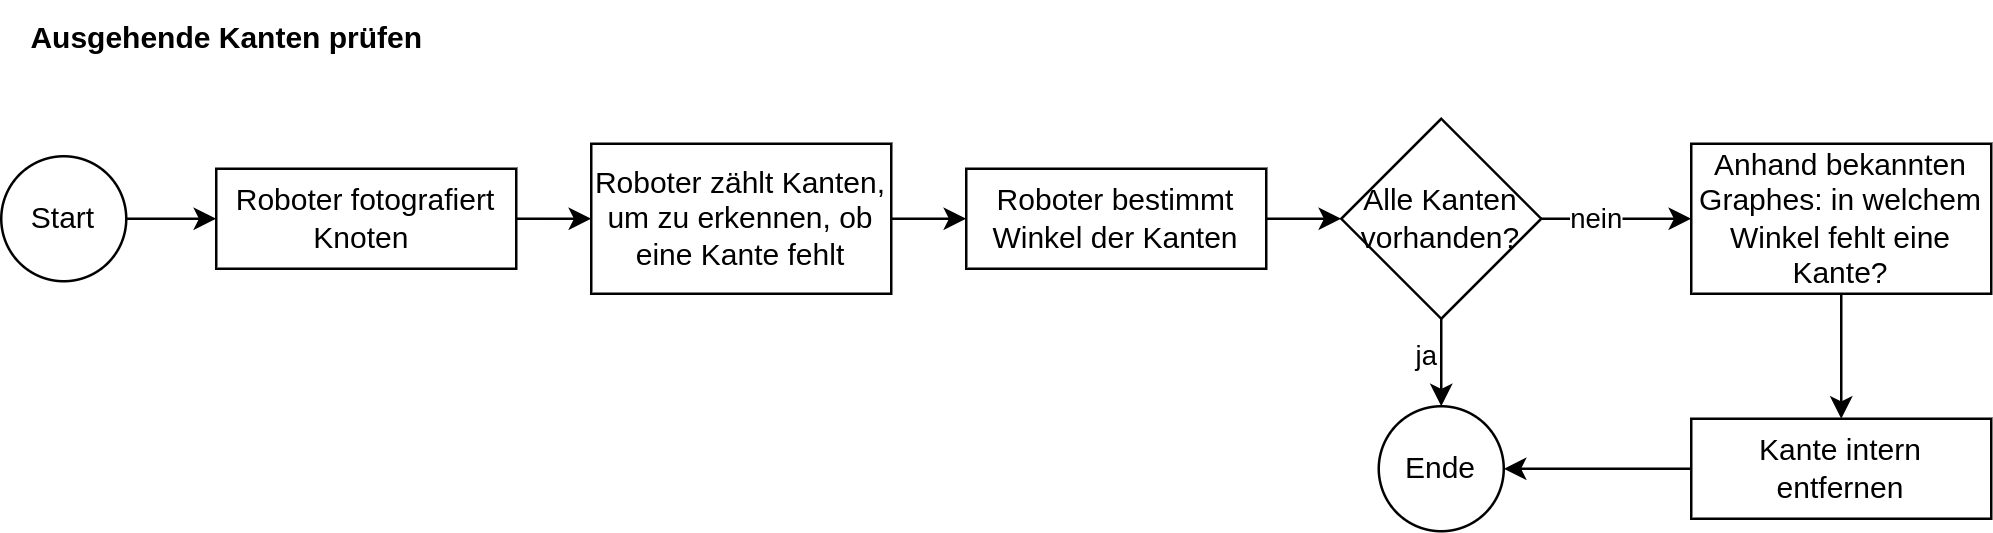
\includegraphics[width=\textwidth]{assets/gesamtkonzept/ablaufdiagramm-kanten-erkennen.png}
\caption{Ablaufdiagramm ausgehende Kanten erkennen}
\label{fig:ablaufdiagramm-kanten-erkennen}
\end{figure}

Der Roboter bewegt sich auf einen Konten zu und haelt 20cm vor dem Knoten an. Der Knoten wird fotografiert und der Roboter faehrt anschliessen auf den Knoten. Das Bild wird mit OpenCV zuerst so verzerrt, dass der Knoten moeglichst gerade von oben dargestellt wird. Danach werden die einzelnen Winkel gemessen. Die Koordinaten werden so angepasst, dass die Linie, von der der Roboter kommt, 0 Grad ist. Dies ist im Prototyping Kapitel im Anhang \ref{winkelerkennung} ausfuehrlicher beschrieben. Das Resultat dieser Objekterkennung soll eine Liste sein mit Winkeln.

TODO Was genau in OpenCV wird verwendet?
TODO Beschreib Winkel messen \& verzerren genauer im Prototyp

TODO: BILD KNOTEN, BILD KNOTEN VERZERRT, BILD WINKEL GEMESSEN

Die erhaltene Liste mit Winkeln wird nun verwendet, um moegliche fehlende Linien zu erkennen und die Winkel intern zu speichern.

Der Roboter selber hat einen Grundgraphen mit Winkeln gespeichert. Diese Winkel ergeben sich aus dem zur Verfuegung gestellten Graph.
Da der Graph nicht genau so aufgeklebt sein wird, wie auf der Skizze, wurden Bereiche definiert, in denen sich die Winkel befinden sollten.

TODO CODE von gespeichert mit Winkel und Ranges. TODO Bild von Graph mit Winkekl und Ranges eingezeichnet, TODO Bild von bestimmten Knoten mit Winkeln und Ranges um Grafik zu erklaeren.

Als erstes wird die Laenge der Liste mit Winkeln gemessen. Wenn sich gleich viele Winkel darin befinden, wie es laut dem Grundgraphen ausgehende Linie haben soll, dann bedeutet das, dass keine Linie fehlt. In diesem Fall werden die internen Winkel aktualisiert mit den tatsaechlichen Werten. 

Falls es weniger Winkel gibt als erwartet, werden die erhaltenen Winkel zu den einzelnen moeglichen Bereichen zugeordnet. In diesem Bereich, dem kein Winkel zugeordnet wurde, fehlt eine Linie. Folglich akutalisiert der Roboter seine internen Informationen: eine Linie wird aus dem Grundgraphen entfernt und die anderen Winkel werden ersetzt mit den gemessenen Werten.

Diese beiden Prozesse sind ebenfalls im Prototyping genauer ausgefuehrt (siehe Anhang \ref{winkelerkennung}).

Nachdem der Roboter den naechsten Knoten berechnet hat, wird der Winkel zur richtigen ausgehenden Kante an die Steuerung gesendet. Der Roboter dreht sich, um auf diese Linie weiterzufahren.

\subsubsection{Zielknoten erkennen}

PLACEHOLDER YOLO/OpenCV? OpenCV right?


\subsubsection{Pylonen und Hindernisse erkennen}


\begin{figure}[H]
\centering
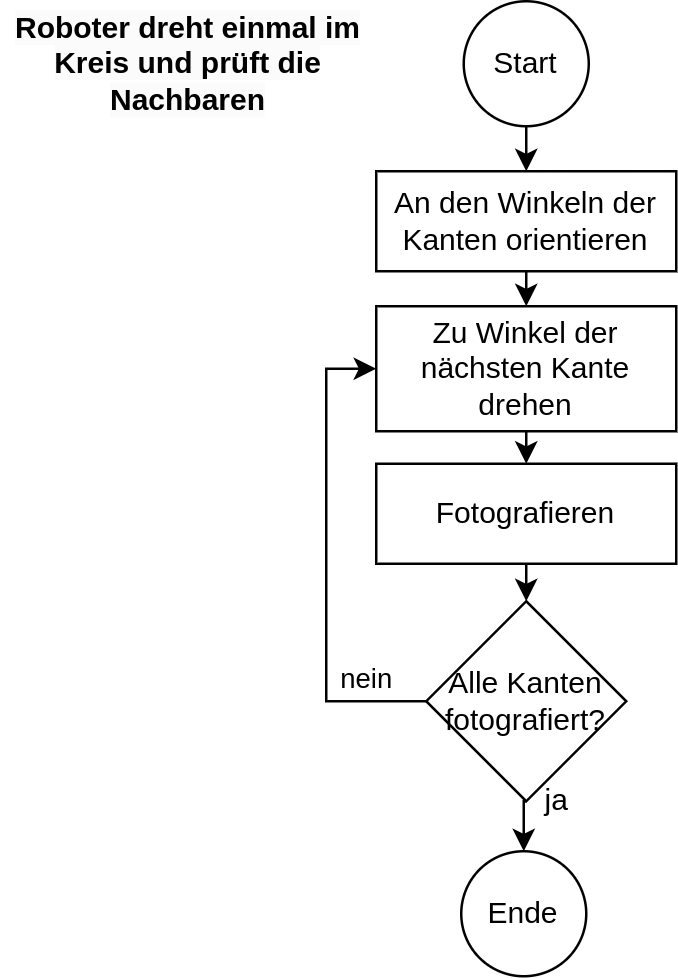
\includegraphics[width=0.35\textwidth]{assets/gesamtkonzept/ablaufdiagramm-hindernisse-erkennen.png}
\caption{Ablaufdiagramm Hindernis erkennen}
\label{fig:ablaufdiagramm-hindernis-erkennen}
\end{figure}

Aus dem vorherigen Schritt der Kanten erkennen, kennt der Roboter alle ausgehenden Linien und deren Position. Er dreht sich nun im Uhrzeigersinn zu jeder Kante und fotografiert diese. Durch das Hochformat der Kameras, sieht er weit und kann auch nur die wichtigen Elemente sehen, sprich, diese, die sich auf der Linie befinden.

Die Bilder werden ausgewertet mit einem YOLO Objekterkennungsalgorithmus. Dabei werden Pylonen und Barrieren erkannt. Beides wird intern gespeichert und bei der Berechnung des Weges beruecksichtigt.

TODO BILDER VON OBJEKTERKENNUNG, Bilder von RASPI in hochformat UND MIT ERKENNUNGEN



\subsubsection{Hindernisse bewegen}

\begin{figure}[H]
\centering
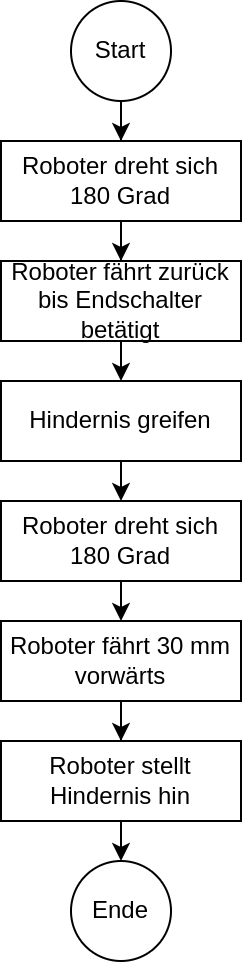
\includegraphics[width=0.4\textwidth]{assets/gesamtkonzept/ablaufdiagramm-hindernis-bewegen.png}
\caption{Ablaufdiagramm Hindernis bewegen}
\label{fig:ablaufdiagramm-hindernis-bewegen}
\end{figure}

In der Nutzwertanalyse (Anhang \ref{nutzwertanalyse}) hat man sich zum Anheben des Hindernisses für ein Klemm-Design entschieden, welches das Hindernis oben an der schmalsten Kante an 3 Punkten greift. Das Hindernis soll mit nur einem Motor sowohl "geklemmt" als auch angehoben werden. Mit einem Ultraschall-Sensor soll das vorhanden sein eines Hindernisses und die ungefähre Distanz bestimmt werden. Zur genauen Bestimmung der Distanz vor dem Greifen wird ein Endschalter verwendet.
Der Greifer wird sich an der Rückseite des Fahrzeugs befinden, der Ultraschallsensor vorne. somit Muss sich das Fahrzeug, nach dem ein Hindernis mittels Ultraschall entdeckt wurde um 180° um das Hindernis anzuheben


\subsection{Schnittstellen zwischen den Kompontenten}



